\section{Rozdělení sítí podle rozsahu}
\label{sec:rozdeleni-siti}
Rozsah sítí obecně závisí na tom, jak velké jsou a jak velkou geografickou či technologickou plochu zabírají.
Mezi kritérie patří čas jak dlouho trvá zprávu na takové síti odeslat a čas šíření celé zprávy, použitá linková technologie.
\subsection{Rozdělení podle rosahu}
\subsubsection{PAN (Personal Area Network)}
Sítě určené pro jednoho uživatele.
Jedná se například o síť vytvořené počítačem nebo mobilem.
Hotspot nebo Bluetooth.
\subsubsection{LAN (Local Area Network)}
Síť určená pro jednu budovu pro zapojení počítačů, ale i mobilů, telefonů, \dots
Připadá na ní většinou jednu veřejná IP adresa.
Vlastníkem sítě bývá zaměstnavatel a uživately bývají zaměstnanci.
Přenosová rychlost závisí na použité technologii v řádek gigabitů.
Čím větší tato síť je, tím větší může být zpoždění při komunikaci po ní.
Technologie zapojení: Ethernet, Wi-FI.
\subsubsection{MAN (Metropolitan Area Network)}
Síť zastřešující území obcí.
Provozovatel bývá poskytovatel.
Využití podsítí a nadsítí.
Nabízí služby DNS do internetu.
Technolgie zapojení: Ethernet, XDSL (Telefonní dráty).
\subsubsection{WAN (Wide Area Network)}
Tvořena napojením sítí LAN a WAN.
V našem případě by se mohlo jednat o službu CZ.NIC.
Nabízí DNS.
Rychlost stovek MB.
Technolgie zapojení: XDSL, FDDI (Optika).
\subsubsection{Internet}
Jedná se o síť WAN propojující všechny sítě (LAN, MAN, WAN) dohromady.
Uživatel má přístup k celému internetu.
\subsection{Topologie sítí}
\subsubsection{P-P (Point to point)}
Propojení dvou počítačů mezi sebou. Užívané pro tiskárny.
\subsubsection{Bus}
Dnes nepoužívaná topologie, která má sice nížké pořizovací náklady, ale také velké rušení, je kolizní.
Je zakončena terminátory mezi kterými se všechny počítače připojují na samotnou síť pomocí jedné linky.
\subsubsection{Ring}
Sopjení je dvořeno dalšími dvěma počítači do kruhu.
Nevznikají kolize, přenos dat je jednoduchý, data ale musí přejít přes mnoho uzlů.
Přenos dat probíhá jedním směrem a výpadek jenoho uzlu vyřadí celou síť.
\subsubsection{Star}
V současnosti hojně používaná na LAN.
Spojení počítačů pomocí switche.
Mezi dvěma stanicemi se nachází akorát jeden hop.
Porcha switche vyřadí celou síť.
Selhání klienta ale nemá vliv.
Nedochází ke kolizím.
\subsubsection{Tree}
Použití u rozsahálejších sítí (Škola).
Prakticky se jedná o spojení několika Star sítí.
Záleží akorát na typu propojení samotných sítí k sobě (Možnost využití Ring nebo další Star).
\subsubsection{Mesh}
Topologie náročná na propojení.
Připojuje každého na každého a používá se obvykle u bezdrátových technologií.
Umožňuje rekonfiguraci při výpadcích.\\
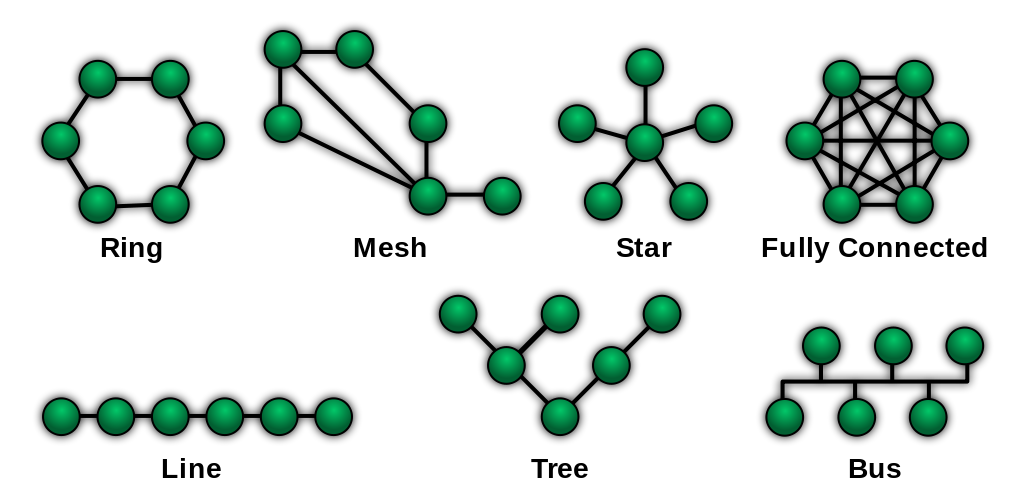
\includegraphics[width=\linewidth]{TVY-POS/Rozdeleni-siti/topologie-siti.png}